\section{Further consideration of fixed wing and hybrid concepts to provide longer endurance during the survey phase of the mission (B.~Phan)}
\label{sec:fixedwing}

After initial flying experiences, it became clear that while the rotorcraft (e.g. quadrotors like DJI Matrice 100 or DJI Mavic Pro Platinum) could take off from a RHIB, fly towards the island, and film, they are limited in range due to the high power cost of hovering flight. Thus, we surveyed additional platforms further, considering fixed wing platforms (which would require arresting gear or similar recovery system), as well as hybrid VTOL platforms envisaged to be launched from the RHIB, fly mostly in an efficient fixed wing configuration, but be capable of vertical recovery onboard. 

\subsection{Rotorcraft}
\begin{figure}
\begin{center}
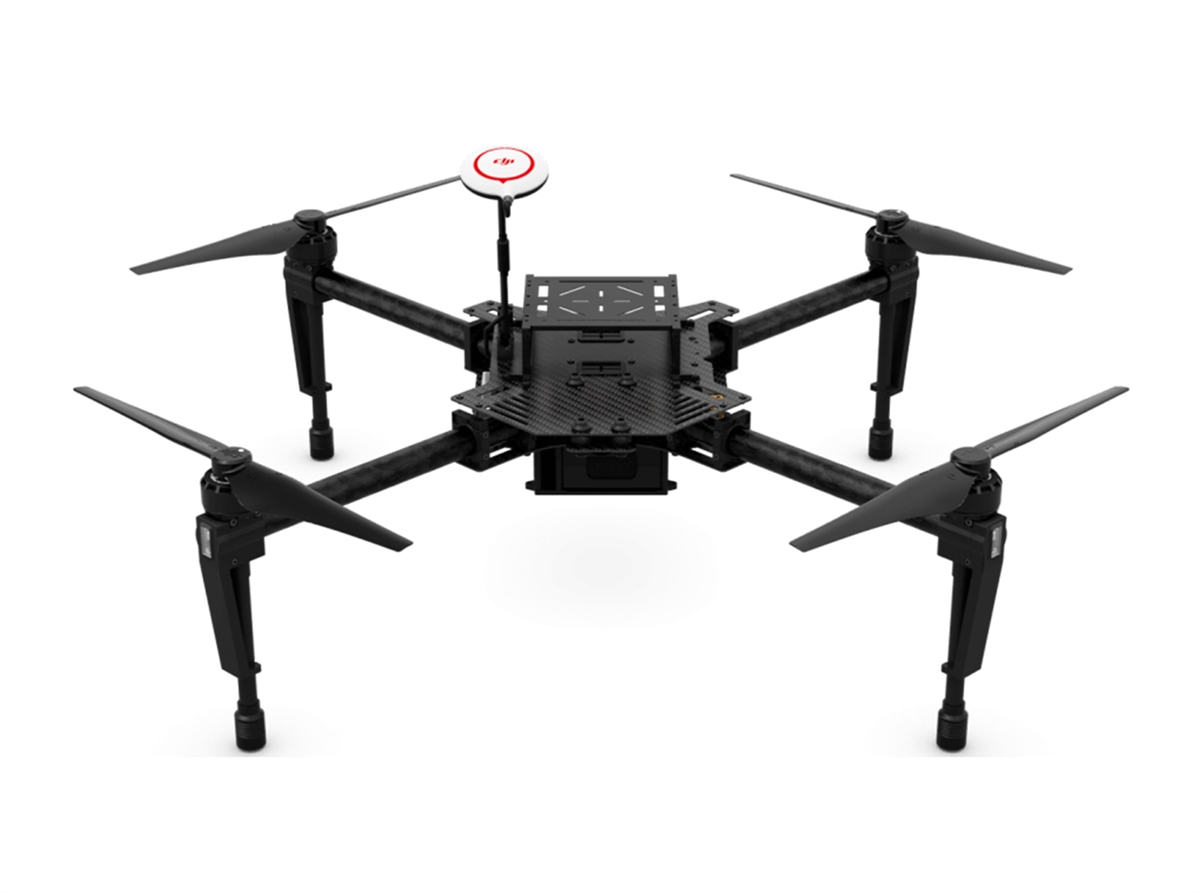
\includegraphics[width=0.49\columnwidth]{figures/survey1.png}
\end{center}
\caption{DJI Matrice 100 (baseline)}
\end{figure}

Platforms discussed: DJI Matrice 100

Platform tested: DJI Matrice 100

Attachments: (DJI Matrice 100) Zenmuse x3 camera, gimbal, TB47D battery, TB48D Battery

Objectives: This platform was our baseline. We wanted to find other systems that had greater endurance, camera quality and maneuverability when landing.

What tests were conducted: Battery life test with the TB87D and TD87D. Camera quality test while in flight. Gimbal maneuverability test. Line of Sight controllability. Reliability with the ground control station.

Landing Procedures Test: Landing operations on a \SI{6x6}{\foot} plank through line of sight (with help from safety observers), internal camera and combination of both.

Lessons Learned: At best with payload of the Zenmuse x3 camera and gimbal the battery would last for about \SI{15}{\minute}. Camera quality while live streaming was ok, when extracted for review it was spotty and glitchy. Gimbal could not yaw, and didn't really have an effect on the mission though because we were still able to angle to our desired locations. Landing was successful but took approximately 1 minutes from the drone being situated directly overhead the boat. Combination of LOS and FPV was best when used to land. FPV was adequate to fly when LOS was not an option. When the remote controller recognized Matice to have critical low battery it would automatically land wherever it was.
 
Recommendations for next year: After testing other systems, the Matrice 100 would not be a good choice for the survey aspect of the mission. Limited endurance and challenges with recovery would give $\sim\SI{10}{\minute}$ of flight time. Furthermore once the ground control station recognized the critical battery the system would auto land. Given a majority of the survey aspect is over water the operators would have to follow the Matrice around the island to mitigate risk of losing the system. Currently we only have 1 on hand. Furthermore given that each battery is $\sim$\$250 it would have been incredibly expensive to constantly change out.

\subsection{Fixed wing}
\begin{figure}
\begin{center}
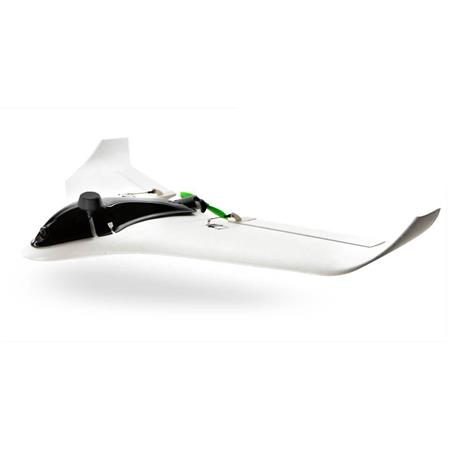
\includegraphics[width=0.49\columnwidth]{figures/survey2a.png}
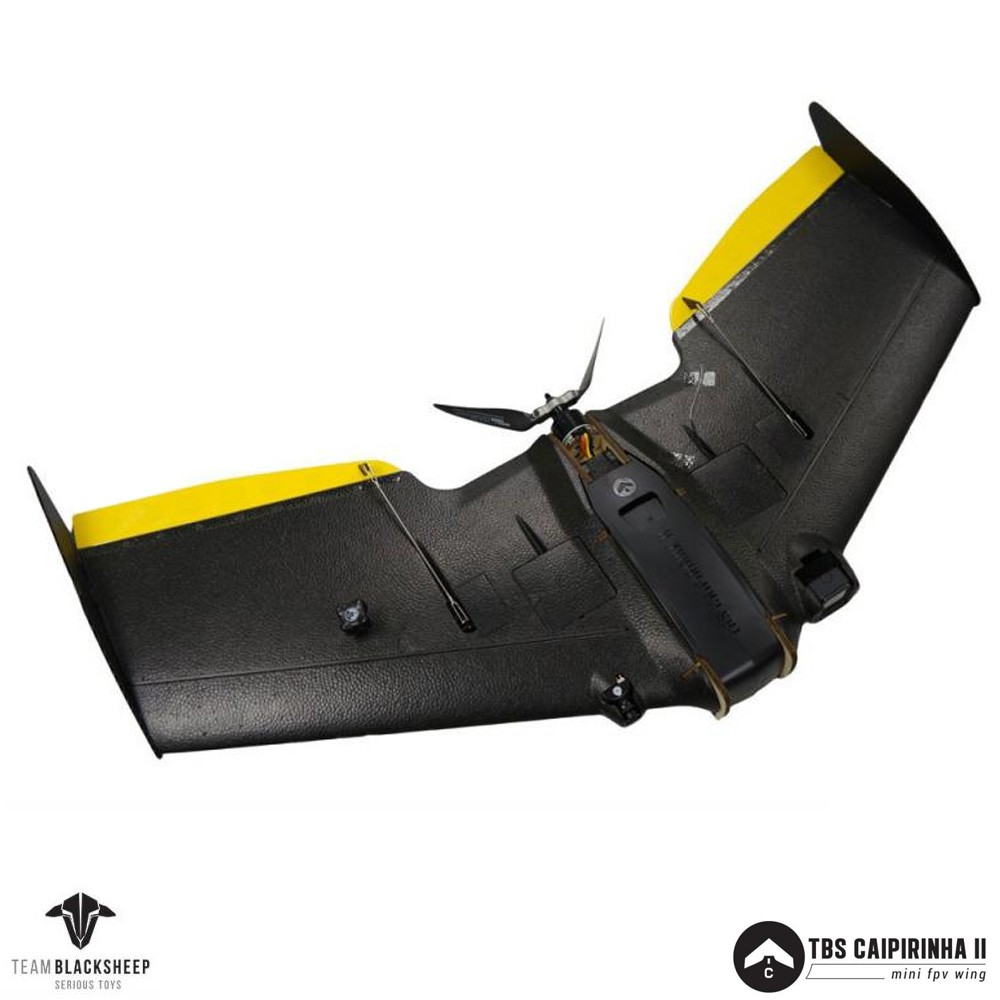
\includegraphics[width=0.49\columnwidth]{figures/survey2b.png}
\end{center}
\caption{Theory Type W. TBS Caipirinha 2}
\end{figure}

Platform: E-Flite Theory Type W, TBS Caipirinha 2

Platform tested: E-Flite Theory Type W

Attachments: (E-Flite Theory Type W) Stock with 4S \SI{1300}{\milli\ampere\hour} Lithium Batteries 

Objectives: Find a system when compared to the Matrice 100 would have longer endurance, better camera quality, autopilot and waypoint capabilities and recoverable from a RHIB.

What tests were conducted: (E-Flite Theory Type W) Practice flying to familiarize myself with the piloting procedures of a fixed wing aircraft. Was buddy-cabled and under the supervision of a licensed UAS trainer with this system for about two flight hours. Practiced different flight modes, launch, intermediate and experienced. Determined proficiency with total amount of hours practiced from someone who had zero experience)

Landing procedure tests: Goal post \SI{10}{\foot} apart with ``net''. Did not test wires and bouncy house methods. 

Lessons Learned: (E-Flite Theory Type W) This specific platform would not be used for the survey aspect of our mission and was tested solely to build proficiency. Starting from zero experience to about two flight hours I would categorize myself as still a beginner. I mainly operated the system in intermediate flight mode. Control of this platform was line of sight in all flights, we did not set up a first person view. After about two hours flight time I am comfortable taking off and doing basic movements such as figure eights and box patterns. However whenever the system was in an uncontrolled state, I did not have the ability to recover and needed to pass control to the UAS trainer. Further when landing the system through the goal post, I was successful 1/10 times collectively from multiple flights. The certified UAS trainer was successful 3/5 times from the same flight. The UAS trainer did this in intermediate mode and recommended this mode for future flights. The goal post was \SI{10}{\foot} apart and \SI{5}{\foot} high on stationary ground. 

(TBS Caipirinha 2) This system was not ordered or live tested in any capacity. However the advertised specifications were promising and worth looking into. The TBS Caipirinha 2 has about \SIrange{45}{90}{\minute} flight time, pre-cut FPV camera, battery, R/C receiver and video transmitter slots. Given the cost for a plug and play version is \$250.

Recommendations for next year: Given that a certified UAS Trainer was only successful recovering the system 3/5 times, I would only recommend this platform to a capable operator with flight experience. The dimensions of the goal post net will be much smaller on the RHIB with the added challenge of not being stationary. (TBS Caipirinha 2) Predicted challenges with this system are: it does not have an autopilot/waypoint function built in, the pre-cut camera slot affords users first person view but we predict that our flight pattern will be the perimeter of the island, meaning the angles would be off and a secondary camera must be installed.







\subsection{Seaplane}
\begin{figure}
\begin{center}
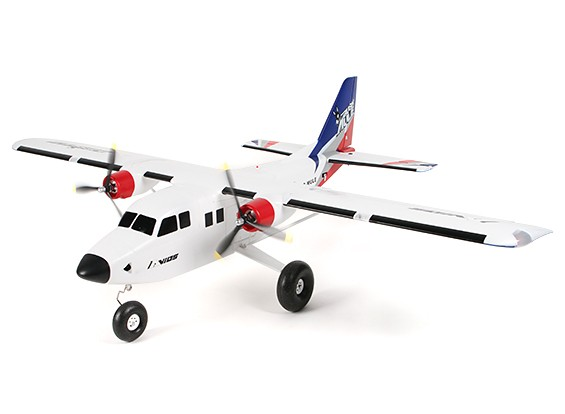
\includegraphics[width=0.49\columnwidth]{figures/survey4a.png}
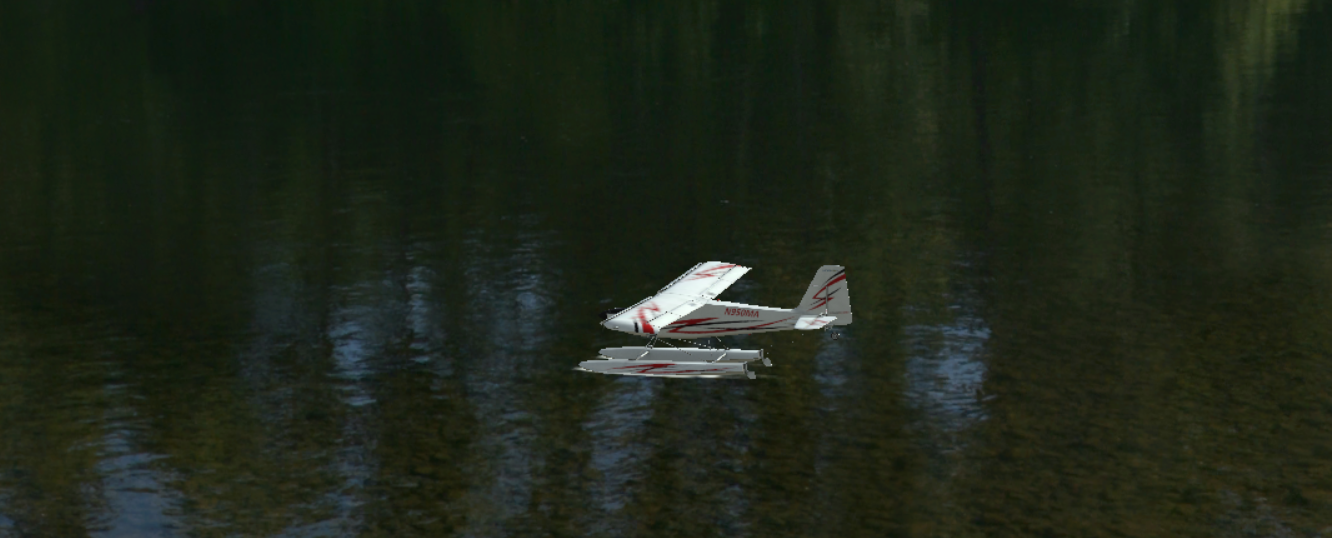
\includegraphics[width=0.49\columnwidth]{figures/survey4b.png}
\end{center}
\caption{Avios Bushmule Seaplane; E-Flite Timber with floats (simulated)}
\end{figure}

Platform: Avios Bushmule (w/o float attachments), E-Flite Timber (with and without float attachment)

Platform tested: Avios Bushmule  (w/o float attachments), E-Flite Timber (simulated in RealFlight 9 program)

Objectives: Find a system when compared to the Matrice 100 would have longer endurance, better camera quality, autopilot and waypoint capabilities and recoverable by a RHIB.

What tests were conducted: (Avios Bushmule) Practice flying to familiarize myself with the piloting procedures of a fixed wing aircraft. Was buddy-cabled and under the supervision of a licensed UAS trainer with this system for about two flight hours. Practiced different flight modes, beginner, intermediate and advanced. Determined proficiency with total amount of hours practiced from someone who had zero experience. Tested my ability to land. Tested the flight time of the system. All tests were conducted line of sight

(E-Flite Timber without float attachments) Practiced flying to gain experience similarly to previous platforms, however used the RealFlight 9 simulation system to complete ``challenges'' that reflected necessary skills for the survey mission. The challenges built into the simulation were called spot landing and air race. Spot landing graded the accuracy a user was able to land on a desired point. Air race practices maneuverability and precision by passing through an array of gates. All tests were conducted line of sight. I did not find an option to access FPV while in ``challenge mode''

(E-Flite Timber with float attachments) Practiced the take off and landing dynamics of a seaplane in water. While in a simulated environment, I wanted to test the differences in technique of land based landing and water based. Test consisted of a mixture of FPV and line of sight.

Landing procedure tests: Avios Bushmule (w/o float attachments) and E-Flite Timber (without float attachment) Tested spot landing at a predetermined area \SI{10x10}{\foot}.

E-Flite Timber (with float attachment) Practice ability to land in water, noted different techniques and dynamics that water based landing required. Attempted to repeatedly land at the same spot.  
Lessons Learned: The Avios Bushmule  (w/o float attachments) was an easier/forgiving plane to pilot. Because it moves slower, I was able to recover from piloting mistakes. With a single battery we were able to get about \SI{15}{\minute} fight time. The system offers additional payload but that was not tested. Discovered landing was relatively similar to other fixed wing platforms.

(E-Flite Timber with and without float attachments) I have about \SI{5}{\hour} flight time in the simulated environment with this type aircraft. I took the lessons covering fundamentals of flight and tried the challenges offered. Even after \SI{5}{\hour} flight time I would categorize myself as a beginner pilot. Flying line of sight is extremely challenging for me. After making piloting mistakes, I would usually be unable to recover. I was only able to reach level 2 on each of the challenges. When landing the (E-Flite Timber with float attachments) the operator must pitch the aircraft upwards slightly and reduce speed on approach. If the aircraft isn't pitch and going too fast, it will nosedive into the water. Furthermore, when the aircraft lands the underbelly gets wet.  

Recommendations for next year: The ability to land airplanes on water is extremely promising, however further research needs to be done regarding the sea state of the landing areas. The lack of endurance of the models we conclude further research needs to be done for longer duration systems. There is a high probability for the system to get wet so waterproofing the camera system may be necessary. 



\subsection{Fixed wing tail sitter VTOL}
\begin{figure}
\begin{center}
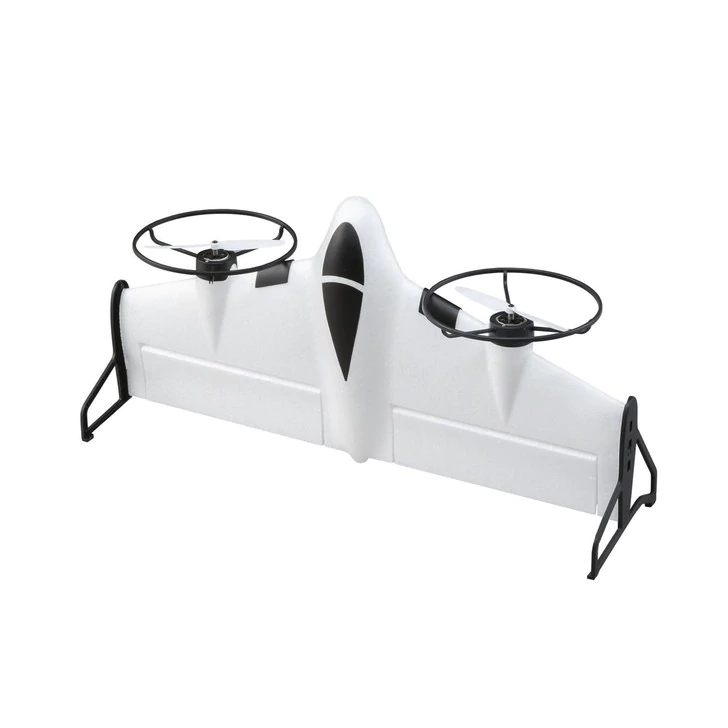
\includegraphics[width=0.49\columnwidth]{figures/survey3a.png}
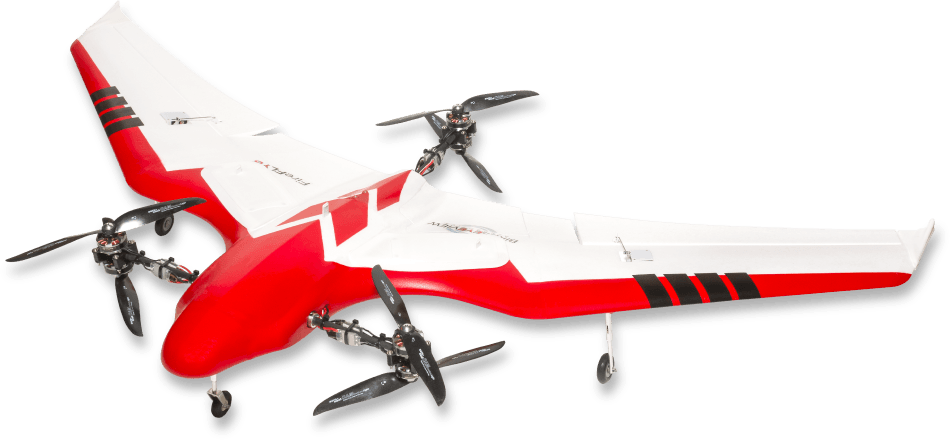
\includegraphics[width=0.49\columnwidth]{figures/survey3b.png}
\end{center}
\caption{E-Flite X-Vert; FireFly 6 Pro}
\end{figure}

Platform: E-Flite X-Vert, FireFLY 6 Pro

Platform tested: E-Flite X-Vert

Attachments: (E-Flite X-Vert) Stock with \SI{800}{\milli\ampere\hour} Lithium Batteries

Objectives: Find a system when compared to the Matrice 100 would have longer endurance, better camera quality, autopilot and waypoint capabilities and recoverable from a RHIB.

What test were conducted: (E-Flite X-Vert) Practice flying to familiarize myself with the piloting procedures of a fixed wing VTOL aircraft. Practiced different flight modes, multirotor, stability and ACRO. Determined proficiency with total amount of hours practiced from someone who had zero experience.

Landing procedure tests: (E-Flite X-Vert) Tested the ability to land in \SI{5x5}{\foot} box both indoor and outdoor. Tested the ability for a person to catch the UAS midair. Tested how the system reacted when held (simulated caught from landing) on full throttle. 

Lessons Learned: The X-Vert is too small to use for the actual mission. It was extremely sensitive to even light windy conditions ($\geq\SI{5}{\mph}$). When in multirotor mode and full throttle the system routinely was unable to fight the strength of the wind and would have to make an emergency landing. These landing were nowhere near the original \SI{5x5}{\foot} box. When in stability mode the system responded better to windy conditions but was still difficult to operate. Noteworthy, when the system was too hard to control, switching back to multirotor mode acted as a failsafe to give inexperienced operators (myself) the ability to hover and regain control.  Indoor tests were successful and we were able to perform touch and gos, ang{360} yaw rotations, and translational movements within the box. Furthermore, Dr. Evangelista (wearing PPE) caught the X-Vert mid-air followed by motor disarm. When Dr. Evangelista held the X-Vert while I attempted to drive it up at full throttle, the system was easily controllable.  I found that the VTOL capabilities were extremely useful in the takeoff and landing aspect of the survey mission. Given a bigger platform this system looks very promising.

(FireFLY 6 Pro) This system has not been tested in any capacity but multiple recently have been ordered by the Weapons department. The advertised specifications prominent to the survey aspect of our mission are; approximately \SI{50}{\minute} flight time from takeoff to landing, can carry a payload of at least \SI{1.25}{\pound}, AvA (Advanced VTOL Autonomy) software that runs on the PX4hawk (aka Pixhawk) autopilot. 

\subsection{Recommendation: VTOL}

Given my inexperience as a UAS operator, I feel the most comfortable piloting VTOL systems. The ability to land like a rotorcraft exponentially lowers the learning curve for newer pilots. Throughout all systems tested I have researched/tested, the FireFLY 6 Pro is the most promising. An expected challenge is that the small area for takeoff and landing is \SI{10x10}{\foot} which is larger than the RHIB we will operate in. 


\subsection{Recommendation: Use of simulators, and early training}

Simulator flights should be the first mastered before attempting to live fly aircraft. I broke both the theory type W and the X-Vert from my inexperience operating a fixed wing system. I have approximately \SI{5}{\hour} of simulated flight time and approximately \SI{2}{\hour} of live flight time and still categorize myself as a beginner. Whenever the system was in an uncontrolled state, I did not have the ability to recover.  I am comfortable taking off and doing basic movements such as figure-eights and box patterns. However when landing strictly fixed wing systems I do not have the capability to accurately pilot the systems through a goal post \SI{10x10}{\foot} wide on a stationary ground. Furthermore, I do not have the capability to land a fixed wing with and without floats repeatedly on a \SI{10x10}{\foot} plot. I do have the capability using VTOL to land on a \SI{6x6}{\foot} stationary plot. Given the volatile nature of the mission having a competent driver is necessary meaning if you want to be the pilot you need to put the hours in! 

If given the chance I would be most confident in piloting the FireFLY 6 Pro. 
       
%
%
%        f you do, write down what you learned and how the procedure changed after trying it in sim - that's important because it's important to know why the steps in a procedure are the way they are
%
%
% and then give metrics of how successful you are at it after n days of training so that future-Phan-wannabes have an idea how long it might take to train for the mission.
%
%
%What did he learn from test flights, 
%develop selection matrix, 
%more detailed preliminary design, etc. If there is an arresting system to be designed, work with MEs to design it; if there is a tail sitter concept, identify type (WingTraOne, stolen from Blount design, etc), same for seaplane. What payload is to be flown, what is its autopilot and which Pixhawk does it need. PArt ordering info, weight and cost estimate if possible.
%
%
%Phan: Concept and preliminary design for the Survey Mission, considering 
%
%
%What did he learn from test flights, develop selection matrix, more detailed preliminary design, etc. If there is an arresting system to be designed, work with MEs to design it; if there is a tail sitter concept, identify type (WingTraOne, stolen from Blount design, etc), same for seaplane. What payload is to be flown, what is its autopilot and which Pixhawk does it need. PArt ordering info, weight and cost estimate if possible.
%  
%e. Somewhere in there I think Lim (maybe with help from Phan) was going to look for a scalign tool or something tog ive first order estimation of range, speed, endurance, payload vs airframe vs battery weight and relationships between these. If you can find a scaling tool and learn how to use it great; if it requires generating some basic scalings via Mathcad (NAOEtype) or Matlab or whatever that works too.